\documentclass[a4paper]{article}

%================================================================================================================================
%
% Packages
%
%================================================================================================================================

\usepackage[T1]{fontenc} 	% pour caractères accentués
\usepackage[utf8]{inputenc}  % encodage utf8
\usepackage[french]{babel}	% langue : français
\usepackage{fourier}			% caractères plus lisibles
\usepackage[dvipsnames]{xcolor} % couleurs
\usepackage{fancyhdr}		% réglage header footer
\usepackage{needspace}		% empêcher sauts de page mal placés
\usepackage{graphicx}		% pour inclure des graphiques
\usepackage{enumitem,cprotect}		% personnalise les listes d'items (nécessaire pour ol, al ...)
\usepackage{hyperref}		% Liens hypertexte
\usepackage{pstricks,pst-all,pst-node,pstricks-add,pst-math,pst-plot,pst-tree,pst-eucl} % pstricks
\usepackage[a4paper,includeheadfoot,top=2cm,left=3cm, bottom=2cm,right=3cm]{geometry} % marges etc.
\usepackage{comment}			% commentaires multilignes
\usepackage{amsmath,environ} % maths (matrices, etc.)
\usepackage{amssymb,makeidx}
\usepackage{bm}				% bold maths
\usepackage{tabularx}		% tableaux
\usepackage{colortbl}		% tableaux en couleur
\usepackage{fontawesome}		% Fontawesome
\usepackage{environ}			% environment with command
\usepackage{fp}				% calculs pour ps-tricks
\usepackage{multido}			% pour ps tricks
\usepackage[np]{numprint}	% formattage nombre
\usepackage{tikz,tkz-tab} 			% package principal TikZ
\usepackage{pgfplots}   % axes
\usepackage{mathrsfs}    % cursives
\usepackage{calc}			% calcul taille boites
\usepackage[scaled=0.875]{helvet} % font sans serif
\usepackage{svg} % svg
\usepackage{scrextend} % local margin
\usepackage{scratch} %scratch
\usepackage{multicol} % colonnes
%\usepackage{infix-RPN,pst-func} % formule en notation polanaise inversée
\usepackage{listings}

%================================================================================================================================
%
% Réglages de base
%
%================================================================================================================================

\lstset{
language=Python,   % R code
literate=
{á}{{\'a}}1
{à}{{\`a}}1
{ã}{{\~a}}1
{é}{{\'e}}1
{è}{{\`e}}1
{ê}{{\^e}}1
{í}{{\'i}}1
{ó}{{\'o}}1
{õ}{{\~o}}1
{ú}{{\'u}}1
{ü}{{\"u}}1
{ç}{{\c{c}}}1
{~}{{ }}1
}


\definecolor{codegreen}{rgb}{0,0.6,0}
\definecolor{codegray}{rgb}{0.5,0.5,0.5}
\definecolor{codepurple}{rgb}{0.58,0,0.82}
\definecolor{backcolour}{rgb}{0.95,0.95,0.92}

\lstdefinestyle{mystyle}{
    backgroundcolor=\color{backcolour},   
    commentstyle=\color{codegreen},
    keywordstyle=\color{magenta},
    numberstyle=\tiny\color{codegray},
    stringstyle=\color{codepurple},
    basicstyle=\ttfamily\footnotesize,
    breakatwhitespace=false,         
    breaklines=true,                 
    captionpos=b,                    
    keepspaces=true,                 
    numbers=left,                    
xleftmargin=2em,
framexleftmargin=2em,            
    showspaces=false,                
    showstringspaces=false,
    showtabs=false,                  
    tabsize=2,
    upquote=true
}

\lstset{style=mystyle}


\lstset{style=mystyle}
\newcommand{\imgdir}{C:/laragon/www/newmc/assets/imgsvg/}
\newcommand{\imgsvgdir}{C:/laragon/www/newmc/assets/imgsvg/}

\definecolor{mcgris}{RGB}{220, 220, 220}% ancien~; pour compatibilité
\definecolor{mcbleu}{RGB}{52, 152, 219}
\definecolor{mcvert}{RGB}{125, 194, 70}
\definecolor{mcmauve}{RGB}{154, 0, 215}
\definecolor{mcorange}{RGB}{255, 96, 0}
\definecolor{mcturquoise}{RGB}{0, 153, 153}
\definecolor{mcrouge}{RGB}{255, 0, 0}
\definecolor{mclightvert}{RGB}{205, 234, 190}

\definecolor{gris}{RGB}{220, 220, 220}
\definecolor{bleu}{RGB}{52, 152, 219}
\definecolor{vert}{RGB}{125, 194, 70}
\definecolor{mauve}{RGB}{154, 0, 215}
\definecolor{orange}{RGB}{255, 96, 0}
\definecolor{turquoise}{RGB}{0, 153, 153}
\definecolor{rouge}{RGB}{255, 0, 0}
\definecolor{lightvert}{RGB}{205, 234, 190}
\setitemize[0]{label=\color{lightvert}  $\bullet$}

\pagestyle{fancy}
\renewcommand{\headrulewidth}{0.2pt}
\fancyhead[L]{maths-cours.fr}
\fancyhead[R]{\thepage}
\renewcommand{\footrulewidth}{0.2pt}
\fancyfoot[C]{}

\newcolumntype{C}{>{\centering\arraybackslash}X}
\newcolumntype{s}{>{\hsize=.35\hsize\arraybackslash}X}

\setlength{\parindent}{0pt}		 
\setlength{\parskip}{3mm}
\setlength{\headheight}{1cm}

\def\ebook{ebook}
\def\book{book}
\def\web{web}
\def\type{web}

\newcommand{\vect}[1]{\overrightarrow{\,\mathstrut#1\,}}

\def\Oij{$\left(\text{O}~;~\vect{\imath},~\vect{\jmath}\right)$}
\def\Oijk{$\left(\text{O}~;~\vect{\imath},~\vect{\jmath},~\vect{k}\right)$}
\def\Ouv{$\left(\text{O}~;~\vect{u},~\vect{v}\right)$}

\hypersetup{breaklinks=true, colorlinks = true, linkcolor = OliveGreen, urlcolor = OliveGreen, citecolor = OliveGreen, pdfauthor={Didier BONNEL - https://www.maths-cours.fr} } % supprime les bordures autour des liens

\renewcommand{\arg}[0]{\text{arg}}

\everymath{\displaystyle}

%================================================================================================================================
%
% Macros - Commandes
%
%================================================================================================================================

\newcommand\meta[2]{    			% Utilisé pour créer le post HTML.
	\def\titre{titre}
	\def\url{url}
	\def\arg{#1}
	\ifx\titre\arg
		\newcommand\maintitle{#2}
		\fancyhead[L]{#2}
		{\Large\sffamily \MakeUppercase{#2}}
		\vspace{1mm}\textcolor{mcvert}{\hrule}
	\fi 
	\ifx\url\arg
		\fancyfoot[L]{\href{https://www.maths-cours.fr#2}{\black \footnotesize{https://www.maths-cours.fr#2}}}
	\fi 
}


\newcommand\TitreC[1]{    		% Titre centré
     \needspace{3\baselineskip}
     \begin{center}\textbf{#1}\end{center}
}

\newcommand\newpar{    		% paragraphe
     \par
}

\newcommand\nosp {    		% commande vide (pas d'espace)
}
\newcommand{\id}[1]{} %ignore

\newcommand\boite[2]{				% Boite simple sans titre
	\vspace{5mm}
	\setlength{\fboxrule}{0.2mm}
	\setlength{\fboxsep}{5mm}	
	\fcolorbox{#1}{#1!3}{\makebox[\linewidth-2\fboxrule-2\fboxsep]{
  		\begin{minipage}[t]{\linewidth-2\fboxrule-4\fboxsep}\setlength{\parskip}{3mm}
  			 #2
  		\end{minipage}
	}}
	\vspace{5mm}
}

\newcommand\CBox[4]{				% Boites
	\vspace{5mm}
	\setlength{\fboxrule}{0.2mm}
	\setlength{\fboxsep}{5mm}
	
	\fcolorbox{#1}{#1!3}{\makebox[\linewidth-2\fboxrule-2\fboxsep]{
		\begin{minipage}[t]{1cm}\setlength{\parskip}{3mm}
	  		\textcolor{#1}{\LARGE{#2}}    
 	 	\end{minipage}  
  		\begin{minipage}[t]{\linewidth-2\fboxrule-4\fboxsep}\setlength{\parskip}{3mm}
			\raisebox{1.2mm}{\normalsize\sffamily{\textcolor{#1}{#3}}}						
  			 #4
  		\end{minipage}
	}}
	\vspace{5mm}
}

\newcommand\cadre[3]{				% Boites convertible html
	\par
	\vspace{2mm}
	\setlength{\fboxrule}{0.1mm}
	\setlength{\fboxsep}{5mm}
	\fcolorbox{#1}{white}{\makebox[\linewidth-2\fboxrule-2\fboxsep]{
  		\begin{minipage}[t]{\linewidth-2\fboxrule-4\fboxsep}\setlength{\parskip}{3mm}
			\raisebox{-2.5mm}{\sffamily \small{\textcolor{#1}{\MakeUppercase{#2}}}}		
			\par		
  			 #3
 	 		\end{minipage}
	}}
		\vspace{2mm}
	\par
}

\newcommand\bloc[3]{				% Boites convertible html sans bordure
     \needspace{2\baselineskip}
     {\sffamily \small{\textcolor{#1}{\MakeUppercase{#2}}}}    
		\par		
  			 #3
		\par
}

\newcommand\CHelp[1]{
     \CBox{Plum}{\faInfoCircle}{À RETENIR}{#1}
}

\newcommand\CUp[1]{
     \CBox{NavyBlue}{\faThumbsOUp}{EN PRATIQUE}{#1}
}

\newcommand\CInfo[1]{
     \CBox{Sepia}{\faArrowCircleRight}{REMARQUE}{#1}
}

\newcommand\CRedac[1]{
     \CBox{PineGreen}{\faEdit}{BIEN R\'EDIGER}{#1}
}

\newcommand\CError[1]{
     \CBox{Red}{\faExclamationTriangle}{ATTENTION}{#1}
}

\newcommand\TitreExo[2]{
\needspace{4\baselineskip}
 {\sffamily\large EXERCICE #1\ (\emph{#2 points})}
\vspace{5mm}
}

\newcommand\img[2]{
          \includegraphics[width=#2\paperwidth]{\imgdir#1}
}

\newcommand\imgsvg[2]{
       \begin{center}   \includegraphics[width=#2\paperwidth]{\imgsvgdir#1} \end{center}
}


\newcommand\Lien[2]{
     \href{#1}{#2 \tiny \faExternalLink}
}
\newcommand\mcLien[2]{
     \href{https~://www.maths-cours.fr/#1}{#2 \tiny \faExternalLink}
}

\newcommand{\euro}{\eurologo{}}

%================================================================================================================================
%
% Macros - Environement
%
%================================================================================================================================

\newenvironment{tex}{ %
}
{%
}

\newenvironment{indente}{ %
	\setlength\parindent{10mm}
}

{
	\setlength\parindent{0mm}
}

\newenvironment{corrige}{%
     \needspace{3\baselineskip}
     \medskip
     \textbf{\textsc{Corrigé}}
     \medskip
}
{
}

\newenvironment{extern}{%
     \begin{center}
     }
     {
     \end{center}
}

\NewEnviron{code}{%
	\par
     \boite{gray}{\texttt{%
     \BODY
     }}
     \par
}

\newenvironment{vbloc}{% boite sans cadre empeche saut de page
     \begin{minipage}[t]{\linewidth}
     }
     {
     \end{minipage}
}
\NewEnviron{h2}{%
    \needspace{3\baselineskip}
    \vspace{0.6cm}
	\noindent \MakeUppercase{\sffamily \large \BODY}
	\vspace{1mm}\textcolor{mcgris}{\hrule}\vspace{0.4cm}
	\par
}{}

\NewEnviron{h3}{%
    \needspace{3\baselineskip}
	\vspace{5mm}
	\textsc{\BODY}
	\par
}

\NewEnviron{margeneg}{ %
\begin{addmargin}[-1cm]{0cm}
\BODY
\end{addmargin}
}

\NewEnviron{html}{%
}

\begin{document}
\meta{url}{/exercices/qcm-bac-blanc-es-l-sujet-4-maths-cours-2018/}
\meta{pid}{10499}
\meta{titre}{QCM - Bac blanc ES/L Sujet 4 - Maths-cours 2018}
\meta{type}{exercices}
%
\begin{h2}Exercice 1 (4 points)\end{h2}
\par
\emph{Cet exercice est un questionnaire à choix multiples (QCM). Les questions sont indépendantes les unes des autres. Pour chacune des questions suivantes, une seule des trois réponses proposées est exacte.  \\Indiquer sur la copie le numéro de la question et la réponse exacte \textbf{en justifiant le choix effectué}. }
\par
\emph{\textbf{Toute réponse non justifiée ne sera pas prise en compte.}}
\par
\begin{itemize}
     \item \textbf{Question 1 :}
     \par
     Soit la fonction $f$ définie sur $\mathbb{R}$ par :
     \[ f(x)=\dfrac{\text{e}^{2x}+1}{\text{e}^{-2x}+1}. \]
     Alors, pour tout réel $x$ :
     \par
     \textbf{a.~~} $f(x)=\text{e}^{2x}$
     \par
     \textbf{b.~~}  $f(x)=\dfrac{1}{\text{e}^{x}}$
     \par
     \textbf{c.~~}  $f(x)=\dfrac{1}{\text{e}^{2x}}$
     \par
     \vspace{5mm}
     \item \textbf{Question 2 :}
     \par
     La courbe $\mathscr{C}_f$ ci-après est la représentation graphique d'une fonction $f$ dans un repère orthonormé.
     \begin{center}
          \begin{extern}%width="400" alt="Courbe représentative Cf"
               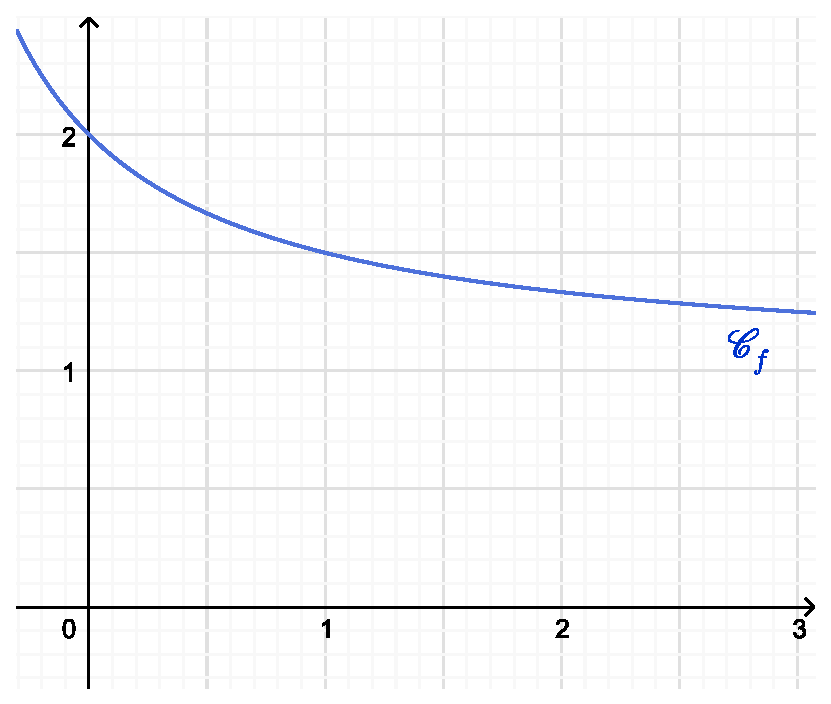
\includegraphics[width=0.7\textwidth]{images/BBESL-s4-1-1}% gbb 1 unite=4cm
          \end{extern}
     \end{center}

\begin{center}
\imgsvg{images/BBESL-s4-1-1}{0.3}% alt="Courbe représentative Cf" style="width:40rem"
\end{center}
     On pose $I= \displaystyle\int_{0}^{2}f(x)\text{d}x$.
     \par
     Alors :
     \par
     \textbf{a.~~} $0 < I < 2$ \\
     \textbf{b.~~} $2 < I < 4$ \\
     \textbf{c.~~} $8 < I < 16$ \\
     \item \textbf{Question 3 :}
     \par
     Soit $g$ la fonction définie sur $\mathbb{R}$ par :
     \par
     \[ g(x)=x \text{e}^{x}+1. \]
     \par
     Alors, pour tout réel $x$ :
     \par
     \textbf{a.~~} $g'(x)=\text{e}^{x}+1$ \\
     \textbf{b.~~} $g'(x)=(1+x)\text{e}^{x}$  \\
     \textbf{c.~~} $g'(x)=\text{e}^{x}$ \\
     \item \textbf{Question 4 :}
     \par
     $f$ est la fonction définie sur l'intervalle $[0~;~5]$ par :
     \[ f(x)=x^3+6x+1. \]
     \par
     et $\mathscr{C}_f$ sa courbe représentative dans un repère orthogonal du plan.
     \par
     Alors, sur l'intervalle $[0~;~5]$  :
     \par
     \textbf{a.~~} La fonction $f$ est concave \\
     \textbf{b.~~} La fonction $f$ est convexe \\
     \textbf{c.~~} La courbe $\mathscr{C}_f$ possède un point d'inflexion \\
     \par
\end{itemize}
\begin{corrige}
     \begin{itemize}
          % =============================================================================================================================
          \item \textbf{Question 1 :}
          \par
          Réponse correcte :\quad\textbf{ a.}
          \par
          On utilise le fait que pour tout réel $x$ : ${\text{e}^{-2x}=\dfrac{1}{\text{e}^{2x}}}$.
          \par
          Alors :
          \par
          $\text{e}^{-2x}+1=\dfrac{1}{\text{e}^{2x}}+1=\dfrac{1}{\text{e}^{2x}}+\dfrac{\text{e}^{2x}}{\text{e}^{2x}}=\dfrac{1+\text{e}^{2x}}{\text{e}^{2x}}=\dfrac{\text{e}^{2x}+1}{\text{e}^{2x}}$.
          \par
          \vspace{2mm}
          Par conséquent :
          \par
          $f(x)=\dfrac{\text{e}^{2x}+1}{\dfrac{\text{e}^{2x}+1}{\text{e}^{2x}}}=(\text{e}^{2x}+1) \times {\dfrac{\text{e}^{2x}}{\text{e}^{2x}+1}}=\text{e}^{2x}$,
          \par
          après simplification par ${\text{e}^{2x}+1}$.
          \par
          \cadre{rouge}{À retenir}{
               Pour tout réel $u$ :
               \[ \text{e}^{-u}=\dfrac{1}{\text{e}^{u}}. \]
          }
          \par
          % =============================================================================================================================
          \item \textbf{Question 2 :}
          \par
          Réponse correcte :\quad\textbf{ b.}
          \par
          La fonction $f$ est positive sur l'intervalle $[0~;~2]$.
          \par
          L'intégrale $I$ est donc égale à l'aire, exprimée en unités d'aire, du domaine délimité par la courbe $\mathscr{C}_f$, l'axe des abscisses, l'axe des ordonnées et la droite d'équation $x=2$.
          \par
          Ce domaine est coloré en vert sur le graphique ci-après ; l'unité d'aire est l'aire du carré tracé en rouge.
          \par
          \begin{center}
               \begin{extern}%width="400" alt="Aire et intégrale"
                    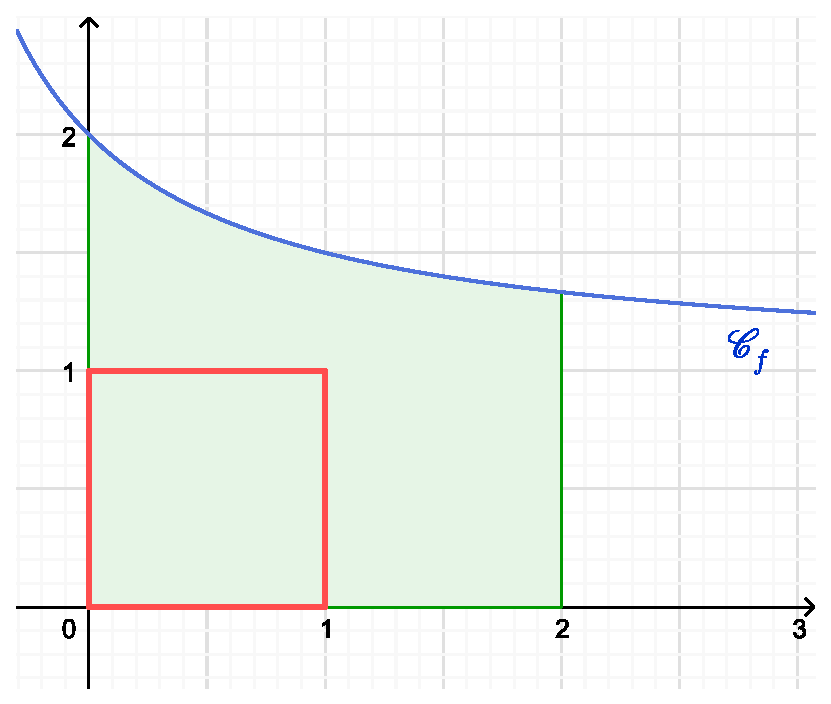
\includegraphics[width=0.7\textwidth]{images/BBESL-s4-1-2}% gbb 1 unite=4cm
               \end{extern}
          \end{center}
          \par
          On voit facilement que l'aire $I$ est comprise entre 2 et 4 unités d'aire.
          \par
          \cadre{rouge}{À retenir}{
               Soit $f$ une fonction définie, continue et \textbf{positive} sur l'intervalle $[a~;~b]$ de courbe représentative $\mathscr{C}_f$.
               \par
               L'intégrale $\displaystyle\int_{a}^{b}f(x)\text{d}x$ est égale à l'aire, en unité d'aire, du domaine délimité par la courbe $\mathscr{C}_f$, l'axe des abscisses, et les droites d'équation $x=a$ et $x=b$.
          }
          \par
          % =============================================================================================================================
          \item \textbf{Question 3 :}
          \par
          Réponse correcte :\quad\textbf{ b.}
          \par
          La dérivée de la fonction constante $x \longmapsto 1$ est nulle.
          \par
          Pour dériver la fonction $x \longmapsto x \text{e}^{x}$ on pose :
          \[ u(x)=x  \qquad \text{et} \qquad v(x)=\text{e}^{x}. \]
          Alors :
          \[ u'(x)=1 \qquad \text{et} \qquad  v'(x)=\text{e}^{x}. \]
          Donc :
          \par
          $g'(x)=u'(x)v(x)+u(x)v'(x)=\text{e}^{x}+x \text{e}^{x}=(1+x)\text{e}^{x}$,
          \par
          après factorisation de $\text{e}^{x}$.
          \par
          %=============================================================================================================================
          \item \textbf{Question 4 :}
          \par
          Réponse correcte :\quad\textbf{ b.}
          \par
          $f$ est une fonction polynôme sur l'intervalle $[0~;~5]$.
          \par
          $f$ et $f'$ sont donc dérivables sur l'intervalle $[0~;~5]$ et :
          \par
          $f'(x)=3x^2+6$ ;
          \par
          $f''(x)=6x+1$.
          \par
          $f''$ est une fonction affine qui est strictement positive sur l'intervalle $[0~;~5]$ (en effet, $6x+1$ est strictement positif dès lors que $x>-\dfrac{1}{6}$).
          \par
          La fonction $f$ est donc \textbf{convexe} sur l'intervalle $[0~;~5]$.
          \cadre{vert}{En pratique}{
               Pour montrer qu'une fonction $f$, deux fois dérivable sur un intervalle $I$ est \textbf{convexe}, on montre que sa dérivée seconde est \textbf{positive} sur $I$.
          }
          \par
     \end{itemize}
\end{corrige}

\end{document}